\chapter{Istniejące rozwiązania i historia rozwoju detekcji obiektów w obrazie wideo} \label{ch:historia}
\subsection*{} \noindent Poniższy rozdział zawiera opis istniejących rozwiązań komercyjnych i niekomercyjnych, z którymi autor miał okazję zapoznać. Dodatkowo dołączono krótką historię rozwoju i opisano sposób wykorzystania ich w trakcie opracowywania rozwiązania będącego tematem niniejszej pracy.

\section{Detekcja obiektów w obrazie wideo}
„Deep Learning” koncentruje się na pięciu podstawowych domenach --- klasyfikacja obrazów, rozpoznawanie mowy, semantyczna klasyfikacja tekstów i rozpoznawanie / detekcja obiektów w obrazie wideo. Z punktu widzenia formalnego wideo jest tylko sekwencją obrazów zmieniających się wraz z upływem czasu. Podejście takie zakwestionował i udokumentował Andej Karpathy --- obecnie [styczeń 2019] zatrudniony jako Director of AI at Tesla.
Jego praca ''Large-scale Video Classification with Convolutional Neural Networks''\cite{KarpathyCVPR14} opisuje sposób detekcji obrazu wideo podobnie do detekcji obiektów \index{CNN}CNN\footnote{CNN --- Convolutional Neural Networks} dla modelowego obrazu. Praca ta jest jakby punktem przełomowym w dziedzinie przetwarzania obrazu --- wcześniejsze rozwiązania bazowały na opisywaniu sklasyfikowanego obrazu zestawem słów go reprezentującym (klasyfikacja)\footnote{bag of words} i decydowaniu przy użyciu algorytmu k-means %\index{k-means} 
oraz SVM %\index{SVM}
\footnote{SVM --- Support Vector Machines} o treści obrazu. Artykuł przedstawia podstawy integracji wszystkich wcześniejszych technik w jeden model CNN. Podejście do analizy obrazu wideo poprzez podzielenie jej na trzy komponenty miało wpływ na wszystkie późniejsze algorytmy przetwarzania obrazu:
\begin{itemize}
    \item połączenie elementów w dziedzinie czasu (interakcje, zmiany i przekształcenia)
    \item adaptatywny rozmiar analizowanego regionu
    \item transfer learning\index{transfer learning}
\end{itemize}
%1st d

Aby zmniejszyć ilość potrzebnej pamięci do budowania modelu, Karpathy ze swoim zespołem jednocześnie przetwarzał tylko jeden film, dodatkowo wstępna obróbka była przeprowadzana na różnych maszynach. Aby zapewnić jednakową długość danych wejściowych klipy pochodzące z YouTube podzielono na półsekundowe sekwencje. Agregacja przewidywanych półsekundowych klipów przypomina testowanie klasyfikacji w dziedzinie czasu - w przypadku obrazu  klatka z początku klipu nawet przedstawiając ten sam obraz po pół sekundzie będzie przedstawiała ten sam obraz po pewnej transformacji. Obiekt na obu klatkach może zostać odkształcony w wyniku przemieszczenia się czy to samego obiektu czy też kamery (przekształcenia izomorficzne), jak również mogą ulec zmianie warunki w których wykonywane jest nagranie (wiatr, deszcz, nasłonecznienie itp.).
Karparhy et al. przedstawiają również nowe podejście do dziedziny czasu (w momencie publikacji) --- aplikują zasady opisujące sieci konwulsyjne do dziedziny czasu i zależności czasowych w wideo. Grupa ramek jest składana razem (grupowana) i staje się obrazem wejściowym do sieci CNN %\index{CNN}. 
Standardowa sieć CNN jako wejście otrzymuje macierz danych --- wysokość, szerokość i kolor (wartości w każdym z trzech składowych). Karpathy i jego zespół rozszerzyli parametry wejściowe i wcześniejszą ramkę umieścili na obecnej --- zachowując rozmiary przekazują podwójną informację o kolorze --- dla obu ramek osobno. Ze względu na scalanie ramek, Karpathy et al. zaproponowali różne strategie realizacji przy założeniu klasyfikowaniu jednej ramki (kombinowanej) jednocześnie. W zależności od tego, które ramki są składane, zespół osiągnął inne rezultaty. Poniższy rysunek przedstawia przyjęte strategie.\\
\begin{figure}[ht]
    \centering
    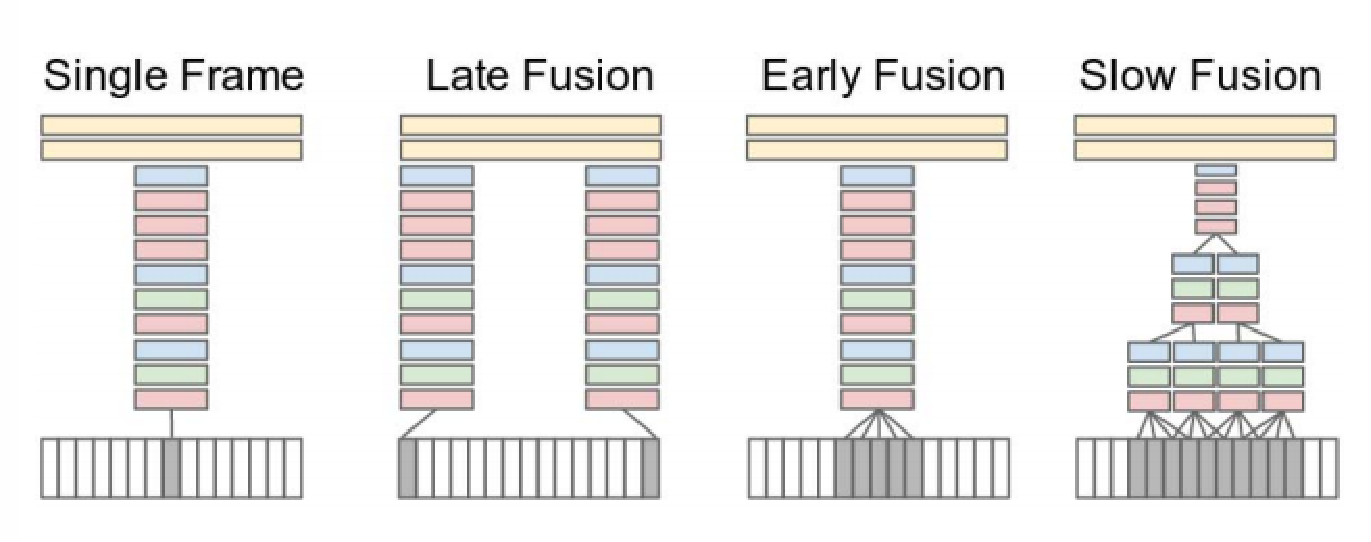
\includegraphics[width=\textwidth]{fig/karpathy1.pdf}
    \caption{Strategie przetwarzania ramek zaproponowane przez Karpathy et al. źródło: ''Large-scale Video Classification with Convolutional Neural Networks''}
    \label{fig:karpathy1}
\end{figure}
\begin{itemize}
\item Model Single Frame z rysunku \ref{fig:karpathy1} reprezentuje wcześniejszy sposób przetwarzania/ klasyfikacji obrazu wideo --- pojedyncza ramka jest interpretowana jak statyczny obraz, informacja temporalna nie jest uwzględniana. 
\item Late Fusion grupuje i scala ramki skraje z zadanego przedziału czasu --- na ostatnią ramkę nakłada się ramkę pierwszą.

\item Early Fusion grupuje kilka ramek z ciągłego przedziału czasu.
\item Slow Fusion jest najbardziej skomplikowanym modelem --- cztery częściowo nakładające się na siebie grupy ramek (ovelapping równy jest dwie ramki) wybrane z ciągłego przedziału czasu są przekształcane przez sieć.
\end{itemize}
W wyniku eksperyment stwierdzono, że Slow Fusion dostarcza najbardziej użyteczną informację o obrazie, jednak jakość ta nie była dużo większa od jakości informacji otrzymanej z modelu Single Frame. Najlepsze wyniki dawało uśrednienie informacji pochodzącej ze wszystkich rozpatrywanych modeli (Single + Early + Late + Slow).
W omawianej pracy przedstawiono również koncept przetwarzana obrazu sieci CNN wielu rozdzielczości.
\begin{figure}[ht]
    \centering
    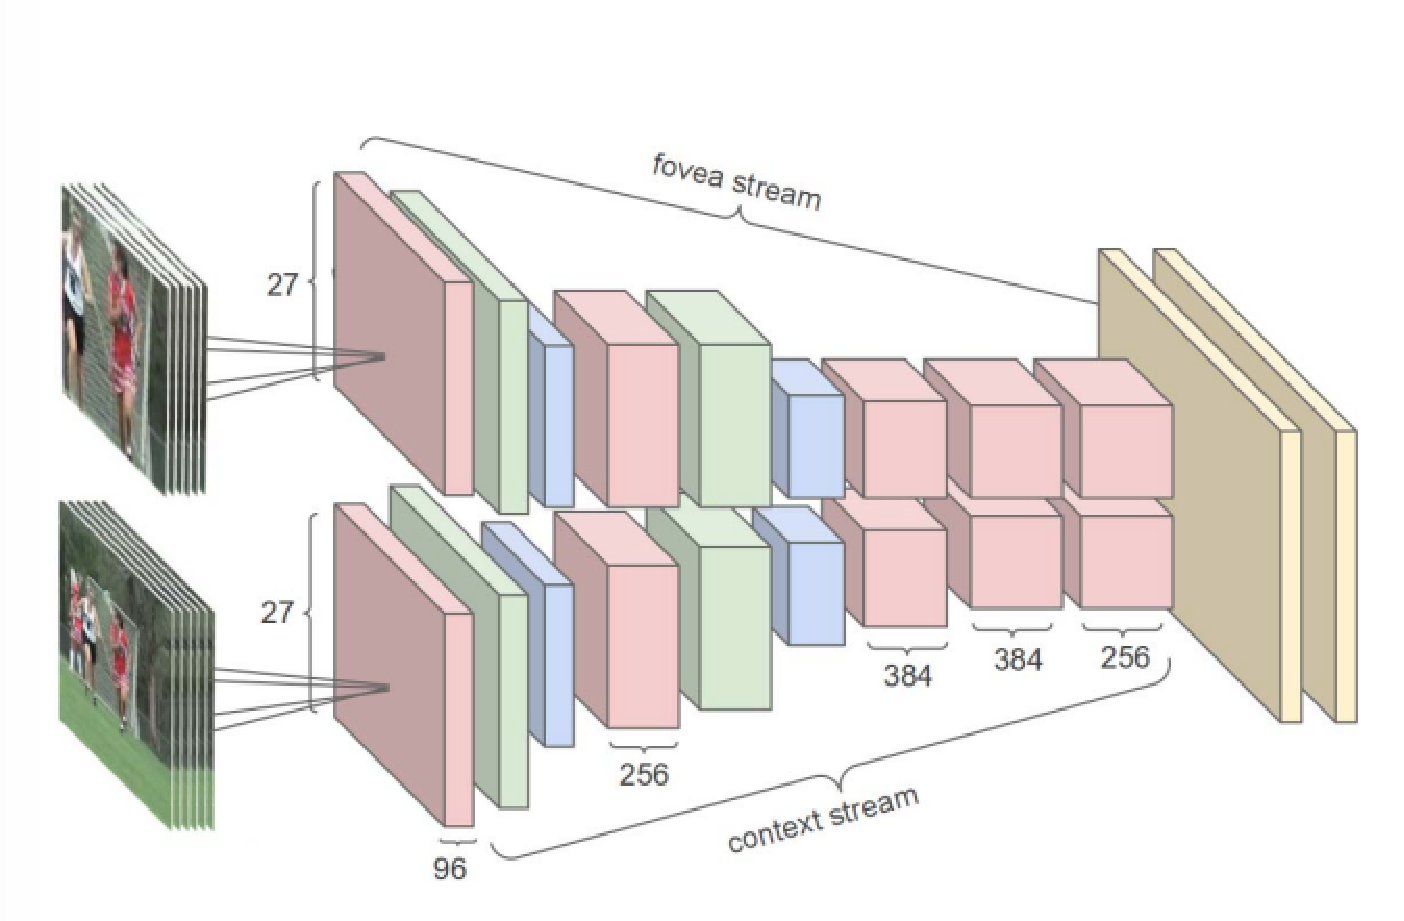
\includegraphics[width=\textwidth]{fig/multi_res.pdf}
    \caption{Strategia klasyfikowania obrazu przez sieci CNN o wielu rozdzielczościach źródło: ''Large-scale Video Classification with Convolutional Neural Networks''}
    \label{fig:multi_resKa}
\end{figure}

Zasada działania przedstawiona na rysunku \ref{fig:multi_resKa} --- dwa odrębne wejścia przetwarzają obraz przez odrębne sieci.

Pomysł przetwarzania wątków o kilku rozdzielczościach polega na jednoczesnym podaniu na wejściu odrębnych sieci neuronowych. Karpathy zaproponował dwa wątki jednocześnie – pierwszy podanie ramki o rozdzielczości 178x178 zdegradowanej do rozdzielczości 89x89 i drugiej ramki wyciętej .ze środka tej samej ramki bazowej o wymiarze 89x89. Oba wątki są sygnałem wejściowym dla odrębnych sieci o budowie Conv-MaxPool-BatchNorm. Zauważony wzrost prędkości w porównaniu do przetwarzania jednego, nie przeskalowanego obrazu wyniósł od 2 do 4 razy. 

Transfer learning.\\

Transfer learning polega na wykorzystaniu przetrenowanej sieci (np. jednego z dostępnych online modelów) i wykonaniu tylko końcowego dostrojenia wag sieci na nowym (docelowym) zestawie danych. Pozwala to na znaczne zaoszczędzenie czasu niezbędnego do trenowania sieci neuronowej jak również pozwala na trenowanie sieci na znacznie mniejszym zestawie danych w porównaniu do tradycyjnego trenowania sieci. Karpathy et al. wykorzystali i opisali dataset Youtube-1M do klasyfikacji zestawy danych UCF-101. Opisany eksperyment objął wykorzystanie 3 warstwowego „transfer learning”. Eksperyment polegał na porównaniu wyników dokładności klasyfikacji dla różnych wariantów sieci. Porównanie umieszczono na rysunku {}. Jak łatwo zaobserwować transfer learning poskutkował prawie 25\% wzrostem dokładności na testowanym zestawie danych. Wyniki eksperymentów przeprowadzonych przez zespół Karpathy et al został uwzględniony w niniejszej pracy.


\section{Rozwiązania i narzędzia}
\subsection{Algorytm Viola---Jones}
\subsection{Dalal i Triggs - HOG}
HOG --- Histograms of Oriented Gradients (2005?)/todo[color=yellow]{Sprawdzić, źródło}
\subsection{CNN}
Deep Learining 2012
\subsection{R---CNN}
\subsection{YOLOv3}
YOLO - You Only Look Once \cite{darkflowwebsite}
\subsection{SSD}
\subsection{Capsule Networks}
\subsection{Tensorflow}
\subsection{Detectron}
\subsection{Darknet}
\subsection{Mask RCNN}
\subsection{OpenVINO toolkit}
\subsection{OpenCV} \todo[color=blue]{Biblioteka i narzedzia do segmentacji obrazu}
\subsection{Python}
\subsection{OpenStreet Map}
\subsection{GIS Server}
\section{Istniejące rozwiązania}
\subsection{Historia}
Historycznie rzecz biorąc pierwszym systemem rozpoznającym znaki drogowe był produkt powstały przy współpracy MobileEye \todo[color=red]{https://www.mobileye.com/} z Continental AG na potrzeby firmy BMW --- system rozpoznawania znaków drogowych dla BMW serii 7. System rozpoznawania znaków od tego czasu
\subsection{NanoNets\cite{nanonets}}